\documentclass{article}
\usepackage{amsmath}
\usepackage{algorithm}
\usepackage{algpseudocode}
\usepackage{physics}
\usepackage{indentfirst}
\usepackage[section]{placeins}

% Language setting
% Replace `english' with e.g. `spanish' to change the document language
\usepackage[english]{babel}

% Set page size and margins
% Replace `letterpaper' with `a4paper' for UK/EU standard size
\usepackage[letterpaper,top=2cm,bottom=2cm,left=3cm,right=3cm,marginparwidth=1.75cm]{geometry}

% Useful packages
\usepackage{amsmath}
\usepackage{graphicx}
\usepackage{subcaption}
\usepackage[colorlinks=true, allcolors=blue]{hyperref}
\usepackage{titling}

\title{Low-Rank Expectile Representations of a Data Matrix, with Application to Diurnal Heart Rates} 
\author{Haytham Tang, Shuge Ouyang, Benjamin Agayre\thanks{Advised by Kerby Shedden}}
\date{}
\begin{document}
\maketitle

\begin{abstract}
    Low-rank matrix factorization is a powerful tool for understanding the structure of 2-way data, and is usually accomplished by minimizing a sum of squares criterion. Expectile analysis generalizes squared-error loss by introducing asymmetry, allowing tail behavior to be elicited. Here we present a framework for low-rank expectile analysis of a data matrix that incorporates both additive and multiplicative effects, utilizing expectile loss, and accommodating arbitrary patterns of missing data. The representation can be fit with gradient-descent. Simulation studies demonstrate the accuracy of the structure recovery. Using diurnal heart rate data indexed by person-days versus minutes within a day, we find divergent behavior for lower versus upper expectiles, with the lower expectiles being much more stable within subjects across days, while the upper expectiles are much more variable, even within subjects.
\end{abstract}

\section{Introduction}
% Researcher Peter Hoff(2010 ish, tensor model/matrix decomposition, first to introduce additive and multiplicative) 
% Matrix model has been widely used for understanding data 2 indices, in particular, here we study models with additive and multiplicative meaning some statistics M = ... 
% GLOVE method. 
% Describing the properties of data

% Briefly introduce the application

% Convey what are expectiles good for, what are low rank representations good for, and why would we combine these ideas?

% Relate this back to the application

Matrix models have been widely employed for understanding data indexed by two variables. In this work, we represent our matrix model as $\mathbf{X}=\mathbf{R} \mathbf{1}^{\top}+\mathbf{1} \mathbf{C}^{\top}+\mathbf{U} \mathbf{V}^{\top}+\mathbf{E}$. In this formula, $\mathbf{R}$  and $\mathbf{C}$ are vectors of row and column effects, representing the heterogeneity in the data. $\mathbf{U}$ and $\mathbf{V}$ are matrices of latent factors, where the outer product $\mathbf{U} \mathbf{V}^{\top}$ captures the higher-order dependencies and clustering patterns. This matrix representation is based on Peter Hoff's additive and multiplicative effects model (AME) \cite{hoff2021additive}. The AME model is capable of capturing various types of statistical dependencies in network data, including node-level correlations, node heterogeneity, and higher-order dependencies such as transitivity and clustering. We apply the AME model to analyze heart rate data with missing values, which comes from a study conducted at RTI International Research Institute
(RTI) in 2016\cite{furberg_2016_53894} capturing 24-hour (circadian) heart rates in 14 human subjects over the course of multiple weeks, obtained using wearable sensors.

In this model, a key contribution is that expectiles are introduced in the setting of matrix factorization. Expectiles are summary statistics that characterize a probability distribution $F$ over a continuum of location parameters, indexed by a value denoted $\tau$ ($0 < \tau < 1$).  Expectiles result from an assymetrically weighted version of ordinary least squares in that the expectile equals the mean when $\tau=1/2$, and in general the expectile minimizes a weighted squared error loss where the positive residuals are weighted by \(\frac{\tau}{1-\tau}\) and the negative residuals are assigned unit weights. For a random variable $X$ with distribution $F$ and a finite first moment, $E|X|<\infty$, Newey and Powell\cite{newey1987asymmetric} introduced expectiles as the set of minimizers:
$$
\mu_\tau:=\arg \min _\mu \int \varsigma_\tau(x-\mu) d F(x)
$$
where the function $\varsigma_\tau$ is an asymmetric least squares criterion:
$$
\varsigma_\tau(u)= \begin{cases}\tau u^2 & \text { if } u \geq 0 \\ (1-\tau) u^2 & \text { otherwise. }\end{cases}
$$


Expectile regression, uses the concept of expectiles to study conditional distributions of an outcome given predictors.  It is an innovative statistical method gaining traction in recent years, and offers a unique approach to analyzing distribution tails. The expectile of a distribution is related to but distinct from the more familiar concept of a quantile. Applications are largely from the field of econometrics, one case in point is in 2021 when Phillips\cite{philipps2021expectile} applied this method to Home Mortgage Disclosure Act data from Boston to find a link between mortgage application cupping and racial disparities. 

Low-rank representations of matrices using expectile loss provide a powerful strategy for handling the vast and complex datasets typical in human data. Low-rank representations are crucial for tasks such as dimensionality reduction, data compression, and noise reduction. They are particularly effective in matrix completion, collaborative filtering, and image processing, enhancing the identification and characterization of circadian patterns in heart rate data. This combination improves the robustness of the analysis against noise and missing data, facilitating the extraction of key features from heart rate data.

% \section{Literature Review}

\section{Model Architecture}
We devised the low-rank model to incorporate both additive effects and UV decomposition. To compare the performance of different optimization algorithms and test the resilience of the model against random initialization, we conducted some simulation studies with preprocessed data generated from the Gaussian Distribution. This section discusses the theoretical derivation of the expectile loss function (and gradients of relevant parameters), the procedure to generate and normalize data and the model fitting implementation. 

\subsection{Expectile Loss Function Derivation}
To calculate the gradient-descent for the low-rank model with additive terms and expectile loss, 
we define $X$ as the feature matrix $n \times p$, $R$ is the $n \times 1$ additive row, $C$ is the $p \times 1$ additive column. $U$ is the $n \times k$ matrix, where $V $ is the $p \times k$ matrix. Then, we can define the following parameters for each non-missing entry:

The predicted matrix is: 
\begin{center}
    $\hat{X} = \hat{R}_{n \times 1}1^{\top}_{p} + 1_{n}\hat{C}_{p \times 1}^{\top} + \hat{U}_{n \times k}\hat{V}^{\top}_{p \times k}$
\end{center}

The residuals are: 
\begin{center}
    $E = X - \hat{X} = X - \hat{R}_{n \times 1}1^{\top}_{p} + 1_{n}\hat{C}_{p \times 1}^{\top} + \hat{U}_{n \times k}\hat{V}^{\top}_{p \times k}$
\end{center}


We can thus define the weight parameter as $W_{ij} = \begin{cases}
    \tau & E_{ij} \geq 0\\
    (1 - \tau) & E_{ij} < 0
\end{cases}$

In order to simplify our expression, we define the mask matrix $M$ which has an indicator value 
\begin{center}
    $M_{ij} = \begin{cases}
    1 & X_{ij} \neq Nan\\
    0 & X_{ij} = Nan
\end{cases}$
\end{center}

Then, we can define the loss function accordingly:
\begin{gather*}
    L = \displaystyle\frac{1}{N}\sum_{i = 1}^{n}\sum_{j = 1}^{p} M_{ij} \cdot W_{ij} \cdot E_{ij}^2\\
\end{gather*}

$W$ is dependent on $E$, we have its partial derivatives with respect to $R/C/U/V$ be either 0 or undefined. In the case when its derivative is $0$, we can simplify expressions and derive the partial derivatives concerning each vector/matrix as:

\begin{gather*}
    \pdv{L}{R} = \pdv{(\frac{1}{N}\sum M \cdot W \cdot E^2)}{R} \\
    = \pdv{(\frac{1}{N}\sum(M \cdot W \cdot (X - \hat{R}_{n \times 1}1^{\top}_{p} + 1_{n}\hat{C}_{p \times 1}^{\top} + \hat{U}_{n \times k}\hat{V}^{\top}_{p \times k})^2))}{R}\\
    = -\frac{2(M \cdot W \cdot (X - \hat{R}_{n \times 1}1^{\top}_{p} + 1_{n}\hat{C}_{p \times 1}^{\top} + \hat{U}_{n \times k}\hat{V}^{\top}_{p \times k}))1^{\top}_{p} + E * 0} {N}\\
    = \frac{-2(M \cdot W \cdot E)1_{p}^\top}{N}
\end{gather*}

\begin{gather*}
    \pdv{L}{C} = \pdv{(\frac{1}{N}\sum(M \cdot W \cdot E^2)}{C} \\
    = \pdv{(\frac{1}{N}\sum(M \cdot W \cdot (X - \hat{R}_{n \times 1}1^{\top}_{p} + 1_{n}\hat{C}_{p \times 1}^{\top} + \hat{U}_{n \times k}\hat{V}^{\top}_{p \times k})^2))}{C}\\
    = \frac{-2(M \cdot W \cdot (X - \hat{R}_{n \times 1}1^{\top}_{p} + 1_{n}\hat{C}_{p \times 1}^{\top} + \hat{U}_{n \times k}\hat{V}^{\top}_{p \times k}))^\top1_{n} + E * 0}{N}\\
    = \frac{-2(M \cdot W \cdot E)^\top1_{n}}{N}
\end{gather*}

\begin{gather*}
    \pdv{L}{U} = \pdv{(\frac{1}{N}\sum(M \cdot W \cdot E^2)}{U} \\
    = \pdv{(\frac{1}{N}\sum(M \cdot W \cdot (X - \hat{R}_{n \times 1}1^{\top}_{p} + 1_{n}\hat{C}_{p \times 1}^{\top} + \hat{U}_{n \times k}\hat{V}^{\top}_{p \times k})^2)}{U}\\
    = \frac{-2(M \cdot W \cdot (X - \hat{R}_{n \times 1}1^{\top}_{p} + 1_{n}\hat{C}_{p \times 1}^{\top} + \hat{U}_{n \times k}\hat{V}^{\top}_{p \times k}))V + E * 0}{N}\\
    = \frac{-2(M \cdot W \cdot E)V }{N}
\end{gather*}

\begin{gather*}
    \pdv{L}{V} = \pdv{(\frac{1}{N}\sum(M \cdot W \cdot E^2)}{V} \\
    = \pdv{(\frac{1}{N}\sum(M \cdot W \cdot (X - \hat{R}_{n \times 1}1^{\top}_{p} + 1_{n}\hat{C}_{p \times 1}^{\top} + \hat{U}_{n \times k}\hat{V}^{\top}_{p \times k})^2))}{V}\\
    = \frac{-2(M \cdot W \cdot (X - \hat{R}_{n \times 1}1^{\top}_{p} + 1_{n}\hat{C}_{p \times 1}^{\top} + \hat{U}_{n \times k}\hat{V}^{\top}_{p \times k}))^\top U + E*0}{N}\\
    = \frac{-2(M \cdot W \cdot E)^\top U}{N}
\end{gather*}

We adopt the partial derivatives above in our loss minimization algorithm. It will be much more complicated when $W$'s partial derivatives concerning $R/C/U/V$ are undefined. We only evaluated and harnessed the calculation of the above gradient in our model. Studies in the future can expand on examining the gradient-descent of a low-rank model for expetile values further. 
\subsection{Data Generation and Preprocessing}
To analyze our model more efficiently, we implemented the following algorithm to generate a simulation dataset drawn from the Gaussian Distribution with thirty percent missing data, which simulates the public dataset of heart rates we have access to.
\begin{algorithm}[H]
\caption{Generate Normal Simulated Data}
\begin{algorithmic}[1]
\Procedure{NormalDataGenerator}{$m, n, r\_sd, c\_sd, u\_sd, v\_sd, \sigma, na\_portion, true\_rank, seed$}
    \State Set random seed to $seed$
    \State $true\_r \gets$ Draw $m$ samples from $N(0, r\_sd)$
    \State $true\_c \gets$ Draw $n$ samples from $N(0, c\_sd)$
    \State $true\_u \gets$ Draw $m \times true\_rank$ samples from $N(0, u\_sd)$
    \State $true\_v \gets$ Draw $n \times true\_rank$ samples from $N(0, v\_sd)$
    \State $\mu\_X \gets true\_r + true\_c + true\_u \cdot true\_v^T$
    \State $error \gets \sigma \cdot m \times n \text{samples from} N(0, 1)$
    \State $X \gets \mu\_X + error$
    \State $missing \gets$ Randomly assign True/False with probability $na\_portion$
    \State Assign $NaN$ to $X$ where $missing$ is True
    \State \Return $X, true\_r, true\_c, true\_u, true\_v$
\EndProcedure
\end{algorithmic}
\end{algorithm}

In this algorithm, parameter $m$ represents the number of rows and $n$ represents the number of columns of the desired data. $r\_sd, c\_sd, u\_sd, v\_sd$ are the standard deviations for each component when drawing samples from the normal distribution, and the standard deviations have default values of 1. Each component is generated separately and the sum is the true feature matrix. $\sigma$ is the standard deviation of error we apply to a standard normal distribution and add to our true $X$. Lastly, we mark $na\_portion$ percentage of our generated data as missing values.

After generating the simulated data, we also applied normalization to the dataset that fits the low-rank model faster with normalized outputs which we can directly compare across trials. The following segment describes the normalization procedure.
\begin{algorithm}
\caption{Normalize Simulated Data}
\begin{algorithmic}[1]
\Procedure{GetNormalizedX}{$X$}
    \State Mask $X$ to ignore $NaN$ values
    \State $mean\_nona \gets$ Compute mean of $X$ ignoring $NaN$
    \State $std\_val \gets$ Compute standard deviation of $X$ ignoring $NaN$
    \State Normalize $X$: $X\_normalized \gets (X - mean\_nona) / std\_val$
    \State Mask $X\_normalized$ to ignore $NaN$ values
    \State Compute row and column means of $X\_normalized$ ignoring $NaN$
    \State \Return $X\_normalized, \text{row means, column means}$
\EndProcedure
\end{algorithmic}
\end{algorithm}

As illustrated above, we first calculated the mean and standard deviation of the data excluding all missing values. We applied normalization to our original data to acquire the normalized data. At this point, we calculated the row means and column means of the normalized data, which will serve as our initialization values for additive factors $R$ and $C$, as discussed in later sections. 
\subsection{Model Fitting}
The next step was to fit our low-rank model with the normalized data. Since we calculated the row means and the column means of the normalized data, we initialized the additive terms $R$ and $C$ with corresponding row means and column means. This initialization reduces some randomness in the effect of $R$ and $C$, and hence focuses more on the initialization effect of $U$ and $V$, which is the main varying component of our model. To initialize $U$ and $V$, we employed the standard normal distribution consistently. 

The initialized parameters were then passed to \textbf{scipy.minimize} method, which updated expectile loss and gradients based on derivations in earlier sections. The underlying optimization algorithm was chosen from \textbf{BFGS, LBFGS,} and \textbf{CG}, whose final loss values and efficiency were evaluated in later sections. The pseudo-code below describes the model fitting procedure, where $X$ is the normalized data, $m$ and $n$ are the number of rows and columns respectively, $\tau$ is the expectile $\tau$ value, and $k$ is the picked rank value for the model. The $\Call{FLATTENPARAMETERS}$, $\Call{UNFLATTENPARAMETERS}$ are methods to manipulate parameter dimensions, and the $\Call{GETOBSERVEDMASK}$ returns where the original data holds non $NaN$ value.
\begin{algorithm}[ht]
\caption{Fitting of Low-Rank Model with Expectile Loss via BFGS/L-BFGS/CG}
\begin{algorithmic}[1]
% I don't think the following pseudocode is necessary to include. Flatten and Unflatten should be 
% straightforward to readers in my opinion -- Haytham
% \Function{GetObservedMask}{$X$}
%     \State \Return $\neg \Call{IsNaN}{X}$
% \EndFunction

% \Function{FlattenParameters}{$R, C, U, V$}
%     \State $U_{flat} \gets \Call{FlattenMatrix}{U}$
%     \State $V_{flat} \gets \Call{FlattenMatrix}{V}$
%     \State \Return $\Call{Concatenate}{[R, C, U_{flat}, V_{flat}]}$
% \EndFunction


% \Function{UnflattenParameters}{$\text{params}, m, n, k$}
%     \State $R \gets \text{params}[:m]$, $C \gets \text{params}[m:m+n]$
%     \State $U \gets \text{params}[m+n:m+n+m \cdot k].\Call{Reshape}{m, k}$
%     \State $V \gets \text{params}[m+n+m \cdot k:].\Call{Reshape}{n, k}$
%     \State \Return $R, C, U, V$
% \EndFunction
\Function{TotalLossAndGradient}{$\text{params}, X, M, \tau, m, n, k$}
    \State $R, C, U, V \gets \Call{UnflattenParameters}{\text{params}, m, n, k}$
    \State $E \gets X - (R[:, \text{np.newaxis}] + C + U @ V^T)$, $E[\neg M] \gets 0$
    \State $W \gets \Call{Where}{E \geq 0, \tau, 1 - \tau}$
    \State $\text{loss} \gets \Call{Sum}{W \cdot E^2} / \Call{Sum}{M}$
    \State $R_{\text{grad}} \gets -2 \cdot \Call{Sum}{W \cdot E, \text{axis}=1} / \Call{Sum}{M}$
    \State $C_{\text{grad}} \gets -2 \cdot \Call{Sum}{W \cdot E, \text{axis}=0} / \Call{Sum}{M}$
    \State $U_{\text{grad}} \gets -2 \cdot (W \cdot E) @ V / \Call{Sum}{M}$
    \State $V_{\text{grad}} \gets -2 \cdot (W \cdot E)^T @ U / \Call{Sum}{M}$
    \State $\text{grad} \gets \Call{FlattenParameters}{R_{\text{grad}}, C_{\text{grad}}, U_{\text{grad}}, V_{\text{grad}}}$
    \State \Return $\text{loss}, \text{grad}$
\EndFunction


\Function{Optimize}{$X, \text{row\_mean}, \text{col\_mean}, k, \tau$}
    \State $m, n \gets \Call{Dimensions}{X}$, $M \gets \Call{GetObservedMask}{X}$
    \State $\text{init\_r\_param} \gets \text{row\_mean}$
    \State $\text{init\_c\_param} \gets \text{col\_mean}$
    \State $\text{init\_uv\_param} \gets \Call{RandomNormal}{0, 1, m \cdot k + n \cdot}$
    \State $\text{params} \gets \text{concatenate}(\{\text{init\_r\_param}, \text{init\_c\_param}, \text{init\_uv\_param}\})$
    \State $\text{result} \gets \Call{Minimize}{\text{TotalLossAndGradient}, \text{params}, (X, M, \tau, m, n, k), \text{'BFGS/L-BFGS/CG'}}$
    \State \Return $R, C, U, V \gets \Call{UnflattenParameters}{\text{result.x}, m, n, k}$
\EndFunction
\end{algorithmic}
\end{algorithm}
\FloatBarrier

\subsection{Result Standardizing}
Finally we standardize the matrix obtained from the decomposition to regularize our model and ensure that the resulting components are more consistent with different randomization of trials. The procedure is described below. We enforce that each column of $V$ has a mean of 0, $U$ is normalized, and $C$ has a mean of 0. This way, we standardize our resulting $R,C,U,V$ from different trials and compare their results. This is useful for subsequent data processing and analysis as it helps to reduce the randomization effect and scale inconsistency in the model.

\begin{algorithm}[ht]
\caption{Standardize Matrix Components}
\begin{algorithmic}[1]
\Require $R, C, U, V$
\Ensure Standardized $R, C, U, V$

\For{$j = 1$ to $\text{number of columns in } V$}
    \State $R \gets R + U[:, j] \times \text{mean}(V[:, j])$
    \State $V[:, j] \gets V[:, j] - \text{mean}(V[:, j])$
\EndFor

\State $U \gets U / \text{norm}(U)$
\State $V \gets V \times \text{norm}(U)$

\State $C \gets C - \text{mean}(C)$
\State $R \gets R + \text{mean}(C)$

\State \Return $R, C, U, V$
\end{algorithmic}
\end{algorithm}
\FloatBarrier

\newpage


\section{Simulation Study}
We carried out a series of simulation studies utilizing the model architecture above to decide which optimization algorithm we would use and analyze our model performance regarding final loss values, mean absolute difference in the recovered data, and the effect of the chosen model rank, all of which paved the way for the analysis of the heart rate data.

\subsection{Simulate Data Configuration}
The heart rate dataset yields a matrix of dimensions $288 \times 334$, corresponding to 288 time bands and 334 person-days. To mirror this structure, our simulated dataset is crafted as a $200 \times 200$ matrix. In the simulation, the standard deviations for $R$, $C$, $U$, and $V$ are set to 1, and the means are set to 0. The simulation incorporates a missing data scheme, in which $30\%$ of the entires in the matrix are missing completely at rancom (MCAR). Furthermore, the matrices $U$ and $V$ possess a true rank of 2. Finally, additive independent Gaussian noise with residual standard deviation $\sigma = 0.3$ is incorporated.

\subsection{Accuracy of the fitted values}

For Mean Squared Error, we understand that the expectile loss value for $\tau = 0.5$ equates to the mean squared error of our prediction. This is given by the expression $\displaystyle\frac{\sigma_{\text{new}}^2}{2}$, where $\sigma_{\text{new}}$ denotes the new error standard deviation post data processing. In our simulated study, we estimate $\sigma_{\text{new}} \approx 0.143$, leading to an expectile loss value of $\displaystyle\frac{\sigma_{\text{new}}^2}{2} \approx 0.0102$. Correspondingly, our model reports a loss value of $0.0098$ when $\tau = 0.5$, which corroborates our theoretical expectations with slightly overfitting. Consequently, this concordance suggests that the model achieves commendable loss values across all $\tau$ levels. The figure below demonstrates our result with 3 different algorithms when we set model rank $k = 2$ and $\tau = 0.5$
\begin{figure}[h]
    \centering
    \includegraphics[width=10cm]{mse_error.jpg}
    \caption{Output of Final Loss Value when $\tau = 0.5$ for 3 algorithms}
    \label{MSE Error}
\end{figure}
\FloatBarrier

\subsection{Comparison of Optimization Algorithms}

In our pursuit to minimize the loss function, we have selected three candidate gradient-based algorithms: Broyden–Fletcher–Goldfarb–Shanno algorithm (\textbf{BFGS}), Limited-Memory Broyden–Fletcher–\\ Goldfarb–Shanno algorithm (\textbf{LBFGS}), and Conjugate Gradient (\textbf{CG}) method. To evaluate the performance and efficiency of these algorithms, we utilized the previously generated simulated data to fit our model, conducting 10 trials for each algorithm. During these trials, we meticulously documented the loss function value at every iteration, alongside the final loss value obtained. Subsequently, we graphed both the raw and logarithmic loss function values, corresponding to a specific expectile $\tau$ and rank $k$.

The aggregated results, depicted in the figure below, reveal distinctive patterns across hundreds of simulations. Notably, the \textbf{BFGS} algorithm exhibits a generally monotonic descent in loss value. Nonetheless, it occasionally encounters periods of stagnation, typically spanning 10-20 iterations, before resuming its downward trajectory. This intermittent stalling contributes to its considerably protracted computation time, typically exceeding that of \textbf{LBFGS} and \textbf{CG} by over a hundredfold. In contrast, the \textbf{LBFGS} and \textbf{CG} methods demonstrate higher convergence rates, with \textbf{LBFGS} outpacing \textbf{CG}. Despite their rapid convergence, both algorithms experience sporadic surges of instability in the loss function values at certain iterations. Ultimately, the final loss values attained by all three algorithms display a high degree of consistency.

Given that the loss values converged by the trio of algorithms are nearly indistinguishable, and considering the markedly reduced computational duration offered by \textbf{LBFGS} in comparison to its counterparts, we have elected to employ the \textbf{LBFGS} algorithm for fitting our model to the public dataset. This decision is predicated on the algorithm's enhanced efficiency in calculating our predictive matrix.

\begin{figure}[h]
    \centering
    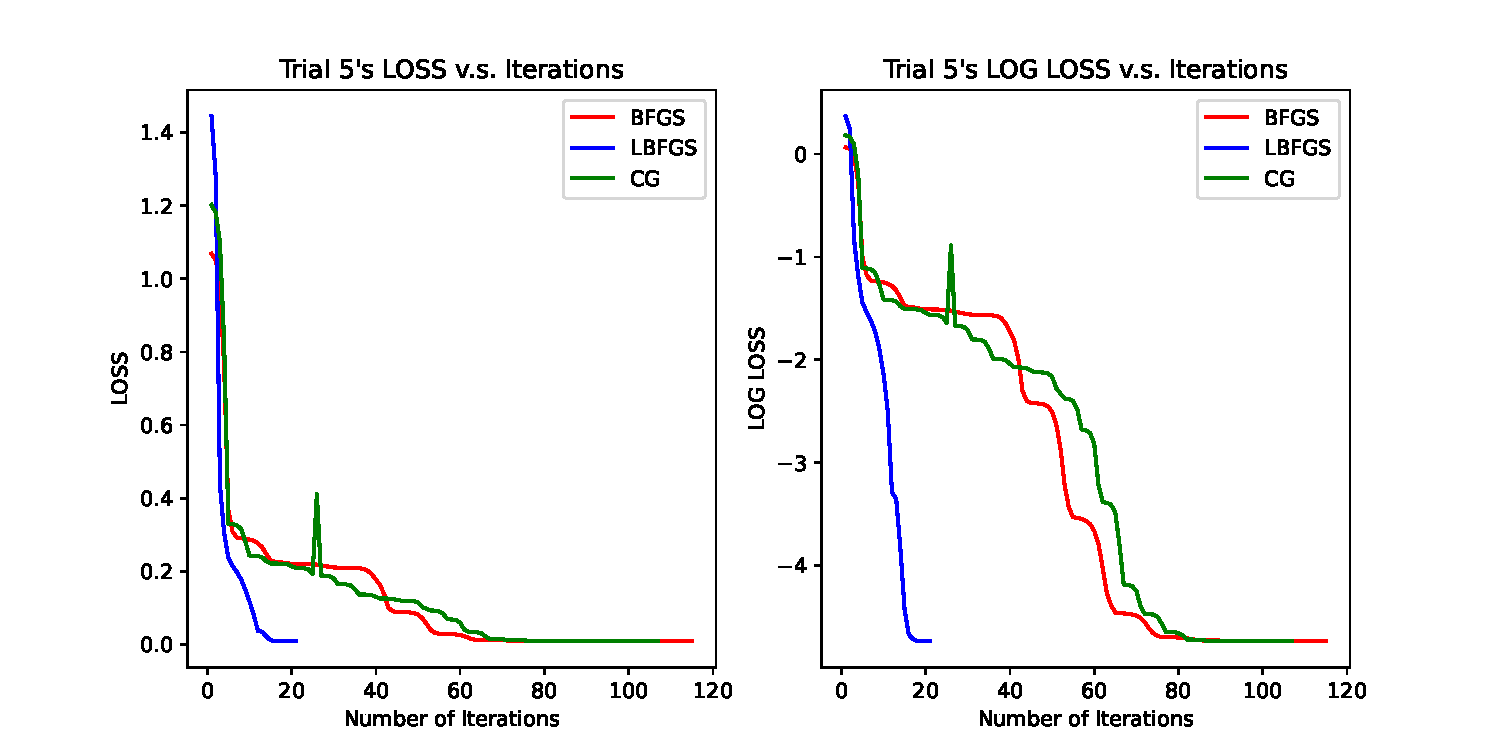
\includegraphics[width=13.5cm]{lossfigure.jpg}
    \caption{Snapshot of Loss Values for 3 Algorithms when $\tau = 0.3$ and $k = 2$}
    \label{Snapshot of Loss Values for 3 Algorithms when $\tau = 0.3$ and $k = 2$}
\end{figure}
\FloatBarrier


\subsection{Resilience of Model to Random Initialization}
After the comparative analysis of the optimization algorithms, we investigated the stability of our model concerning varying initial conditions. For each trial, the matrices $R$ and $C$ were initialized utilizing the constant row and column means, respectively, obtained from the data preprocessing phase. Conversely, the matrices $U$ and $V$ were initialized randomly following a Standard Normal Distribution. We executed a set of 10 trials, within which we evaluated the discrepancies in the final loss values and computed the mean absolute difference for each pair of trials, culminating in a total of 45 comparative assessments. This procedure enabled us to produce heatmaps that illustrate these comparisons for each algorithm, akin to the figure presented subsequently.

\begin{figure}[h]
    \centering
    \includegraphics[width=16cm]{heatmap.jpg}
    \caption{Heatmap of Difference of Final Loss Value and Mean of Absolute Difference of 45 Pairs}
    \label{Heatmap}
\end{figure}
\FloatBarrier

The outcomes depicted above suggest that the variability in the final loss values between trial pairs is on the order of $10^{-7}$, while the mean absolute difference between trials lies in the order of $10^{-3}$. These findings positively demonstrate the model's robustness against random initializations, affirming its efficacy in reliably reconstructing data with a high degree of stability across multiple iterations.

\subsection{Effect of misspecification of model rank}
In our simulation study, we further explored the impact of the selected model rank on the loss value. Our findings indicate that when the true rank of $U$ and $V$ is denoted as $x$, and the chosen model rank $k$ is less than this true rank ($k < x$), the resultant final loss value significantly exceeds the anticipated range, deteriorating further as $k$ decreases. Conversely, when the selected model rank $k$ meets or surpasses the true rank ($k \geq x$), the final loss values align closely with expectations. However, it is noteworthy that the optimization duration escalates with an increase in $k$.

For instance, consistent with the previous discussion, the true rank of the simulated data's $U$ and $V$ matrices is 2. We conducted simulations across different ranks $k = 1, 2, 3, 4$ with a constant $\tau = 0.1$. The empirical outcomes, depicted in the subsequent figures, demonstrate that the final loss values for $k = 1$ are approximately an order of magnitude greater than those obtained for $k = 2, 3, 4$. Furthermore, while the loss values for $k = 2, 3, 4$ exhibit remarkable consistency, the computational time required by the algorithm significantly increases with slight overfitting for $k = 3$ and $4$, compared to the true rank of 2.

These observations can be rationalized by acknowledging that a model rank lower than the true rank leads to an underspecified model with insufficient parameters, introducing systematic bias and manifesting as an under-fitted model with elevated loss values. In contrast, a model rank exceeding the true rank results in an overspecified scenario where the model, burdened by an excess of parameters, necessitates extended periods to minimize loss, yet ultimately converges to a loss value that mirrors the expected outcome.

\begin{figure}[h]
    \centering
    \includegraphics[width=10cm]{k=1.jpg}
    \caption{Result when $k = 1, \tau=0.1$}
    \label{k=1}
\end{figure}
\begin{figure}[h]
    \centering
    \includegraphics[width=10cm]{k=2.jpg}
    \caption{Result when $k = 2, \tau=0.1$}
    \label{k=2}
\end{figure}
\begin{figure}[h]
    \centering
    \includegraphics[width=10cm]{k=3.jpg}
    \caption{Result when $k = 3, \tau=0.1$}
    \label{k=3}
\end{figure}
\begin{figure}[h]
    \centering
    \includegraphics[width=10cm]{k=4.jpg}
    \caption{Result when $k = 4, \tau=0.1$}
    \label{k=4}
\end{figure}

\FloatBarrier
\section{Heart rate Data Modeling}

\subsection{Dataset Overview}
The dataset for our analysis comes from a study conducted at RTI International Research Institute (RTI) in 2016 \cite{furberg_2016_53894}.  The data were subsequently hosted on the Kaggle platform.   Thirty subjects were recruited and given FitBit Fitness Trackers, which capture 24 hour heart rates as well as other parameters.  Here we focus on the 14 subjects with reported heart rate data over multiple days.

The Fitbit monitor records heart rates every five seconds.  We segmented the 24 hour day into 288 segments of five minute duration, and used the median of all recorded heart rates within each five minute segment for each person day as a summary for analysis.  Segments with no available data are treated as missing.  This yields data for 14 people and a total of 334 person days.  Within these days the overall proportion of missing segment values is $29.8\%$.

Heart rates largely follow a circadian pattern with a nadir (daily minimum) early in the morning, a rapid rise after awakening, a plateau or bimodal pattern in mid day, and a gradual decline in the evening.  However a wide variety of person day deviations from this typical pattern may occur, for example due to work schedules, difference between weekends and week days, and individual differences associated with lifestyle and demographics.

We first inspected the raw data, and calculated some descriptive statistics of the recorded heart rates.  In particular, we used the marginal expectiles to summarize the heart rate distribution over all person days, for each time segment.  This was done for 9 different values of $\tau$ to capture a wide range of the distribution.

\begin{figure}[ht]
  \centering
  \begin{subfigure}[b]{0.48\textwidth}
    \includegraphics[width=\textwidth]{1 person-day.png}
    \label{fig:sub1}
  \end{subfigure}
  \hfill
  \begin{subfigure}[b]{0.49\textwidth}
    \includegraphics[width=\textwidth]{expectile heartrate.png}
    \label{fig:sub2}
  \end{subfigure}
  \caption{Left: recorded heart rates for one observed person-day.  Right: marginal expectiles for each segment, over all person days.}
  \label{fig:example}
\end{figure}

From the right panel of figure \ref{fig:example}, we observe that
the circadian heart rate pattern is broadly similar across all $\tau$ values, with the curves being translated vertically with increasing $\tau$.  However the curves for different values of $\tau$ are notably more compressed at around the time of morning awakening and more dispersed throughout the afternoon.  Furthermore, the difference in heart rates tends to be greater between the upper expectiles compared to the lower expectiles, reflecting a right skew in the marginal heart rate distribution.

According to the simulation study, \textbf{LBFGS} is the best optimization algorithm among the three algorithms we tested. We first fit the low-rank model with $\tau = 0.5$ and number of feature equals 1 since this would gives the most stable result. We run this algorithm repeatedly and record the R, C, U, and V for the minimum loss case, and we use these predictions as the start point for other $\tau$ values.

One situation that arises as a result of the model is the occurrence of outlier in the predicted value of V, see figure \ref{outlier}.
This is due to the fact that some columns in our initial matrix have too many missing values. We remove the columns that have more than $70\%$ of the missing value in the matrix, which remains 299 columns. We re-fit the model as described above and got the expected results.

\begin{figure}[ht]
\centering
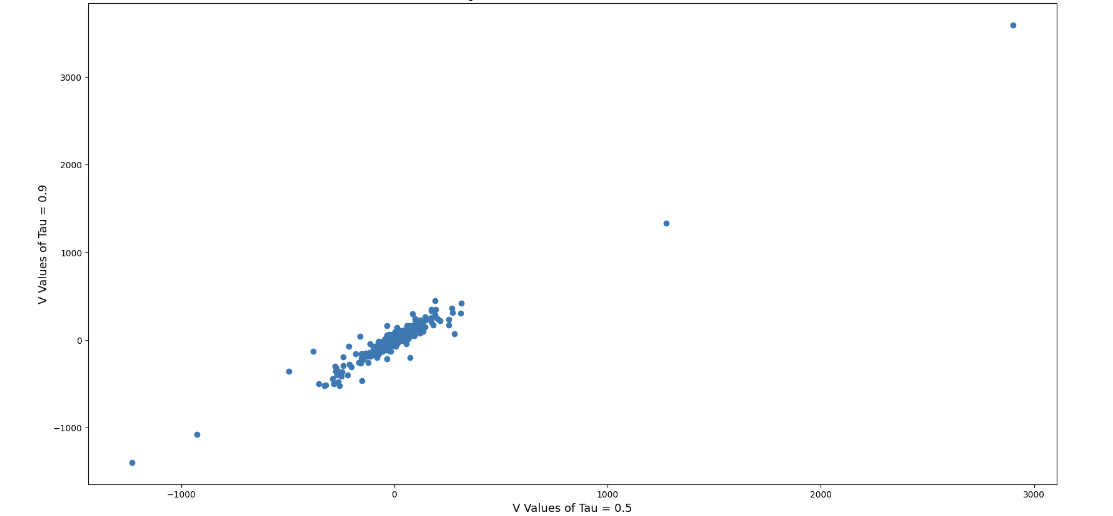
\includegraphics[width=16cm]{outlier.png} 
\caption{LBFGS's Resulting Normalized and Oriented V when $\tau = 0.5$ v.s. $\tau = 0.9$} 
\label{outlier} 
\end{figure}



\subsection{Result Analysis}
\subsubsection{Loss Value Interpretation}
Based on our model, it results in a final loss value of around 0.2658 when $\tau = 0.5$. Since the dataset has a standard deviation of $\sigma \approx 16$, we recover the average difference value between our predicted values and actual values is $\displaystyle\sqrt{0.2658 * 2 * 16^2} \approx 11.667$. This means that with MSE, our predicted heart rate value is 11.667 away from the actual value.\\

On the other hand, when $\tau = 0.9$, the final loss value is around $0.1826$, and multiplying that by the variance gives us 46.75. When $\tau = 0.1$, the final loss value is around $0.094$, and multiplying that by the variance gives us 24.064. We are not certain how to interpret these two values at this point and are open to discussion. 

\subsubsection{Graph Analysis}
The trend of the model-predicted fluctuations in R and U over time over the course of a day for the three $\tau$ values is shown in figure \ref{fig:test}.
\clearpage
\begin{figure}[ht]
  \centering
  \begin{subfigure}[b]{0.45\textwidth}
    \includegraphics[width=\textwidth]{U-Time.png}
    \label{pre-U}
  \end{subfigure}
  \hfill
  \begin{subfigure}[b]{0.48\textwidth}
    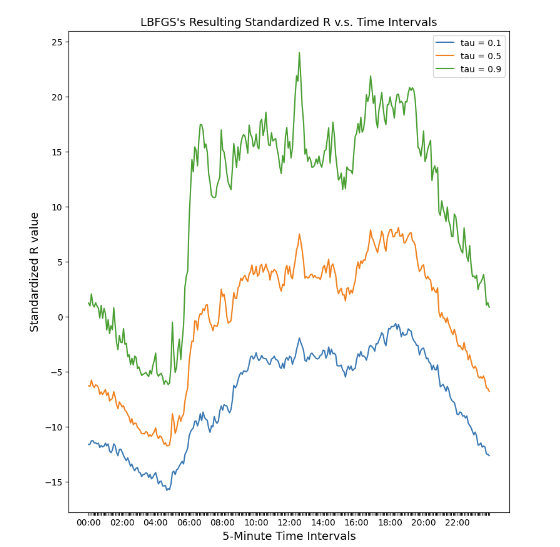
\includegraphics[width=\textwidth]{R-Time.png}
    \label{pre-R}
  \end{subfigure}
  \caption{Result of $R$ and $U$ in different $\tau$ values}
  \label{fig:test}
\end{figure}

The U-matrix usually represents the strength or activity of an implied feature or factor at different points in time, and it is observed in the figure \ref{fig:test} that all three curves show some degree of volatility, which implies that the strength of the implied feature varies at different points in time. Different values of $\tau$ seem to affect the volatility of U . For example, when $\tau$ is 0.1 and 0.9, the fluctuations in U values are more intense most of the time, while for the intermediate $\tau$ value of 0.5, the volatility seems to be slightly flatter.

The values of R over time show a certain pattern that may be related to an underlying trend in the time series data. All three curves show a similar trend between approximately 08:00 and 16:00, suggesting that R at different expectile levels may be influenced by the same temporal factors. In the curve for $\tau = 0.1$, there are many spikes that may indicate the occurrence of a special event, such as a violent activity.

\clearpage
\begin{figure}[ht]
  \centering
  \begin{subfigure}[b]{15cm}
    \centering
    \includegraphics[width=15cm]{V 0.5,0.1.png} 
    \label{fig:sub1}
  \end{subfigure}
  \hfill
  \begin{subfigure}[b]{15cm}
    \centering
    \includegraphics[width=15cm]{V 0.9,0.1.png}
    \label{fig:sub2}
  \end{subfigure}
  \hfill
  \begin{subfigure}[b]{15cm}
    \centering
    \includegraphics[width=15cm]{V 0.9,0.5.png}
    \label{fig:sub3}
  \end{subfigure}
  \caption{Scatter Plot of Resultant $V$ between pair of $\tau$ values}
  \label{fig:V}
\end{figure}
\FloatBarrier
The scatter plots above represent the relationship between the V values for each of the expectile ($\tau = 0.1, 0.5, 0.9$) conditions, see figure \ref{fig:V}.
It can be seen that after deleting some of the columns with high missing rates, the problem of outlier that occurs with the V values is solved and all three scatter plots show a clear positive correlation. This means that the value of V at one value of $\tau$ has a strong linear relationship with the value of V at another value of $\tau$. This linear relationship is stronger in $\tau = 0.1/0.9 \text{ vs. } \tau = 0.5$ and weaker in $\tau = 0.1 \text{ vs. }  \tau = 0.9$. The range of scatter plots varies with $\tau$ value, and at $\tau$ values of 0.1, 0.9, the data points have a wider scatter, implying a greater difference in V between extreme $\tau$ values.

\subsubsection{Intraclass Correlation Coefficient Analysis}
ICC (Intraclass Correlation Coefficient, $\mathrm{ICC}=\frac{\operatorname{Var}(E[Y \mid G])}{\operatorname{Var}(Y)}$) values usually range from 0 to 1, and can be used to assess the consistency of team members in certain performances. 

In our project, we calculate ICC values for each individual's C and V predictions separately to analyze how consistent each person's prediction in our model is under different $\tau$ values. We made a new dataframe for ICC calculation by combining the V and C matrices of the model prediction results with the person Id and detection date corresponding to each index, see figure \ref{icc}.

\begin{figure}[ht]
\centering
\includegraphics[width=0.7\textwidth]{ICC_df.png} 
\caption{Head of the ICC Analysis Dataframe} 
\label{icc} 
\end{figure}

By taking $Y = \textit{C/V}$ and $ G = \textit{each person}$, we get the ICC values of C and V in our model for different $\tau$.
The results of ICC of C at $\tau$ of 0.1, 0.5, and 0.9 are: 0.918, 0.883, 0.646. This shows that predicted $C$ had higher ICC values in all three conditions, especially at $\tau = 0.1 $ and $\tau = 0.5$, indicating strong consistency across individuals for the model fitting. As the $\tau$ value increases, the consistency decreases significantly but still maintains a good level of consistency.

However, at $\tau=0.1,0.5,0.9$, the ICC values of predicted $V$ are  0.406, 0.348,0.285; the ICC values for predicted $V$ are significantly lower than those for predicted $C$ in all three $\tau$ values. This suggests that the within-group consistency of predicted $V$ is relatively low regardless of $\tau$. This low consistency is more pronounced as $\tau$ increases, suggesting that there may be more internal error.
\bibliographystyle{alpha}
\bibliography{cite}

\end{document}